\chapter{Tecnologie}
In questo capitolo verranno descritte le attività preliminari per la realizzazione di questo progetto, le tecnologie utilizzate
unitamente alle motivazioni legate all'uso di questi sistemi rispetto ad altri.

\section{Strutture dati gerarchiche}
Le tabelle di un database relazione non sono gerarchiche (come nel XML), ma sono delle semplici liste piatte. I dati gerarchici sono 
constituiti da relazioni padre-figlio che non possono essere rappresentate in modo naturale nelle tabelle dei database relazionali.
In questo caso, i dati gerarchici sono una collezione di informazioni dove ogni item ha un solo padre e nessuno o più figli
(ad eccezione del nodo radice che non ha un nodo padre); questo genere di rappresentazione delle informazioni può essere trovato in 
diversi ambiti di applicazione di un database, incluse discussioni su forum e mailing list, grafici di organizzazione di un business, 
categorie per gestire contenuti e categorie di prodotti. \\

\newpage

\begin{figure}[H]
	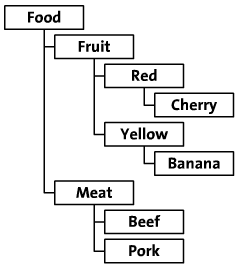
\includegraphics[scale=0.7]{images/Hierarchical_Data_ex.PNG}
	\caption{Esempio di una gestione di dati in modo gerarchico}
	\label{fig:Hde}
\end{figure}

Ci sono differenti modelli per poter gestire dati in modo gerarchico, i più importanti che sono stati presi in considerazione sono i 
seguenti:

\subsection{The adjacency list model}
Il primo approccio, e quello di più semplice implementazione, qui descritto è chiamato \textit{‘adjacency list model} o metodo ricorsivo;
è definito tale perchè per funzionare necessita solo di una funzione che itera per tutto l'albero.\\
In questo modello, ogni item (nodo dell'albero) nella tablla contiene un puntatore al suo item padre; invece il nodo radice avrà un puntatore a un valore
NULL per l'item padre.

\begin{figure}[ht!]
    \centering
	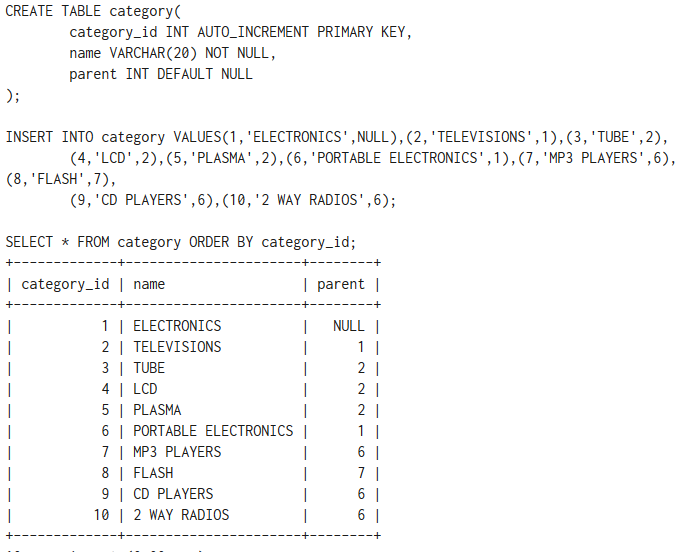
\includegraphics[scale=0.75]{images/Adjacency_list_model_table.PNG}
	\caption{Esempio di una tabella per gestire dati in modo gerarchico secondo l'adjacency list model }
\end{figure}
 
Il vantaggio di usare questo modello sta nella sua semplicità di costruzione sopratutto a livello di codice client-side, 
e di restituzione dei figli di un nodo. Mentre diventa problematico se si lavora in puro SQL e nella maggior parte dei linguaggi di 
programmazione, è lento e poco efficente, perchè è necessaria una query per ogni nodo dell'albero, e visto che ogni query impiega 
un certo periodo di tempo, questo rende la funzione molto lente quando si lavora con alberi di grandi dimensioni.
Inoltre molti linguaggi non sono ottimizzati per funzioni ricorsive. Per ogni nodo, la funzione inizia una nuova istanza di se stessa,
ogni istanza occupa una porzione di memoria e impiega un certo tempo per inizializzarsi, e più grande è l'albero e più questo 
processo sarà portato a termine in maggior tempo.

\subsection{The Nested set model}
Il secondo approccio che viene proposto è il \textit{Nested set model}, che permette di osservare la gerarchia in un modo diverso, non 
come nodi e linee, ma come container innestati. \\

\begin{figure}[ht!]
    \centering
	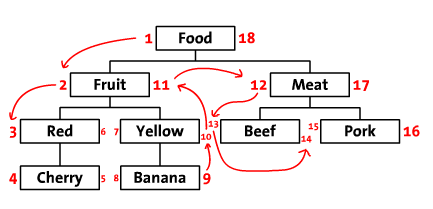
\includegraphics[scale=0.55]{images/Nested_Tree_Model_ex.PNG}
	\caption{Esempio di una gestione di dati in modo gerarchico secondo il Nested set model}
\end{figure}

La gerarchia dei dati viene rappresentata nella tabella attraverso l'uso degli attributi 'left' e 'right' per rappresentare l'annidamento
dei nodi (il nome delle colonne: left e right, hanno significati speciali in SQL; per questo motivo si identificano questi campi con i 
nomi 'lft' e 'rght'). 
Ogni nodo dell'albero viene visitato due volte, assegnando i valori in ordine di visita, e in entrambe le visite. Quindi vengono 
associati ad ogni nodo due numeri, memorizzato come due attributi. 
I valori di left e right sono determinati come segue: si inizia a numerare a partire dal lato più a sinistra di ogni nodo e si continua 
verso destra. Lavorando con un albero, si parte da sinistra e si continua verso destra, un livello alla volta, scendendo per ogni
nodo i suoi figli, assegnando i valori al campo left, prima di assegnare un valore al campo right, e successivamente si continua verso 
destra. Questo approccio è chiamato Modified preorder tree traversal algorithm.

A prima vista questo approccio può sembrare più complicato da comprendere rispetto all'adjacency list model, ma quest'utlimo metodo è
molto più veloce quando si vuole recuperare i nodi, visto che basta una query, mentre più lento per operazioni di aggiornamento e 
cancellazione dei nodi; in quest ultimo il grado di complicatezza dell'operazione è determinato dal nodo che si vuole cancellare, a 
partire dal caso più semplice, il nodo foglia (nodo senza figli) fino al caso più complicato, quando si vuole cancellare il nodo radice. \\

\begin{figure}[ht!]
    \centering
	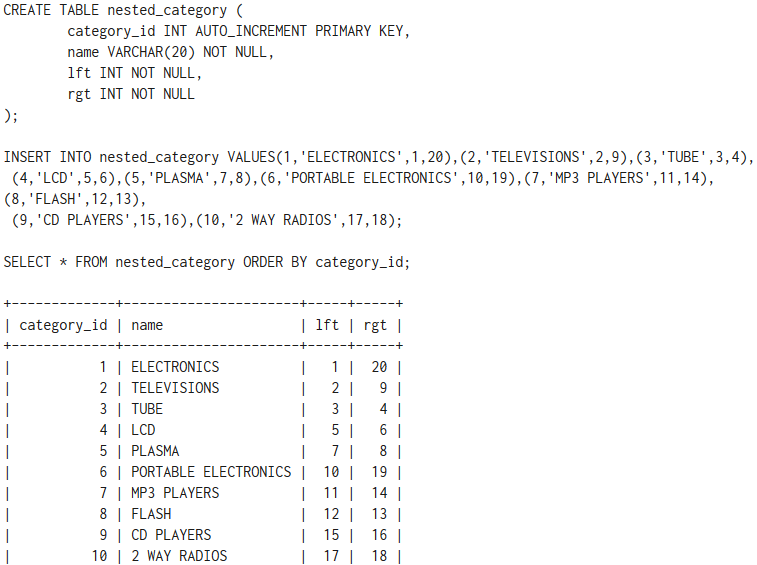
\includegraphics[scale=0.6]{images/Nested_Tree_Model_table.PNG}
	\caption{Esempio di una tabelle per la gestione di dati in modo gerarchico secondo il Nested set model}
\end{figure}

\newpage

\section{Sistemi di raccomandazione}





Recommendation system is a system which recommends items to users among a large number of existing items 
in database. Item is anything which users consider, such as product, book, and newspaper. There is expectation 
that recommended item are items that  user will like most; in other words, such items are in accordance with 
user’s interest. 
There are two common trends of recommendation systems: content-based filtering (CBF) and collaborative 
filtering (CF) as follows [1, pp. 3-13]: 
- CBF recommends an item to a user if such item is similar to other items that she/he likes much in the 
past (her/his rating for such item is high). Note that each item has contents which are properties and so 
all items compose a so-called item content matrix. 
- CF recommends an item to a user if her/his neighbors (other users similar to her/him) are interested in 
such item.  Note  that  user’s  rating  on  an item  expresses  her/his  interest.  All users’  ratings  on  items 
compose a so-called rating matrix. 
Both of them (CBF and CF) have their own strong points and weak points. Namely CBF focuses on content of 
item and  user’s own interest;  it recommends  different  items  to different  users. Each  user  can  receive unique 
recommendation; so this is the strong point of CBF. However CBF doesn’t tend towards community like CF. As 
items that user may like “are hidden under” user community, CBF has no ability to discover such implicit items. 
This is the most common weak point of CBF. 
If  there are a  lot  of  content associating with  item  (for  example, items has  many  properties)  then, CF 
consumes much system resource and  time  in order to analyze items  whereas  CF  doesn’t regard to content  of 
items.  That  CF only works  on  users’  ratings  on  items  is  strong  point  because CF  doesn’t  encounter  how to 
analyze rich content items. However it is also weak point because CF can do unexpected recommendation in 
some situations that items are considered to be suitable to user but they don’t relate to user profile in fact. The 
problem gets more  serious when there are  many items  that aren’t  rated  and  so rating  matrix becomes spares 
matrix containing many missing values.

\begin{figure}[ht!]
	\centering
	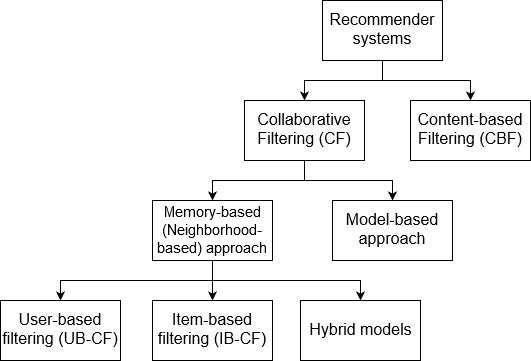
\includegraphics[scale=0.5]{images/recommender_systems.jpg}
	\caption{}
	\label{fig:RS}
\end{figure}


\cite{model-based-approach-for-collaborative-filtering}
Un sistema di raccomandazione filtra i dati usando differenti algoritmi e raccomanda gli item più rilevanti agli utenti,
attraverso un procedimento a 3 fasi:

\begin{description}
	\item[raccolta di dati]: questa è il primo step e anche quello più importante per poter costruire un sistema di 
	raccomandazione che produca risultanti rilevanti e consistenti. I dati possono essere raccolti in due modi: esplicitamente,
	cioè attraverso i dati che vengono prodotti direttamente dagli utenti, ad esempio le valutazioni di un prodotto; mentre 
	attarverso l'approccio implicito, vengono raccolti dati che non sono prodotti in modo intenzionale dall'utente ma raccolti
	dai costanti flussi di dati come la cronologia di ricerca, i click effettuati, lo storico degli ordini, etc.
	\item[memorizzazione di dati]: la quantità di dati definisce quanto efficace un modello di raccomandazione possa di
	diventare. Ad esempio, in un sistema di raccomanzione per film, maggiori sono le valutazioni fornite dagli utenti, e 
	migliore sarà il sistema di raccomandazione per gli altri utenti. Il tipo di dati che si vuole raccogliere determina
	anche il supporto di memorizzazione più adatto.   
	\item[Filtraggio dei dati]: dopo la fase di raccolta e memorizzazione dei dati, essi vanno filtrati per poter estrarre
	le informazioni rilevanti per poter effettuare le raccomandazioni finali, e sono già disponibili diversi algoritmi che
	semplificano quest ultima fase. 
\end{description}

I sistemi di raccomandazione possono essere suddivisi nelle seguenti categorie, ma speso si preferisco degli approcci imbridi cioè delle
combinazioni di sistemi di raccomandazione basati sul contenuto (\textit{Content-based filtering}) e 
quelli collaborativi (\textit{Collaborative filtering}) in modo da essere più efficaci sfruttando i pregi di entrambi gli approcci.


\subsection{Content-based filtering}
Un Content-based filtering è un sistema di raccomandazione in cui vengono suggeriti item simili a un particolare item (oggetti 
o prodotti). 

Questo approccio sfrutta i metadati dell'item, che possono essere il genere, una descrizione, uno o più autori, la categoria di 
appartenenza etc. per fare queste raccomandazioni; l'idea base che sta dietro questi raccomandatori, è che se ad un utente piace 
o interessa un particolare item allora gli piaceranno anche altri item simili.

Questo algoritmo suggerisce prodotti che piacevano all'utente nel passato ed è limitato a item dello stesso tipo. Un 
content-based recommender fa riferimento a quegli approcci, che provvedono raccomandazioni comparano la rappresentazione del
contenuto che descrive un item e la rappresentazione del contenuto dell'item interessato dall'utente. 

Questi metodi sono usati quando si sanno a priori delle informazioni sugli item che si vuole suggerire, ma non sugli utenti.
In questo sistema, delle keyword (parole chiave) sono utilizzate per caratterizzare gli item e un profilo dell'utente è 
costruito per indicare quali item gli piacciono. In altre parole, questi algoritmi cercano di raccomandare item che 
all'utente sono piaciuti o ha usato nel passato e sta esaminando nel presente. La costruzione del profilo dell'utente,
spesso temporaneo, non viene basata su un modulo di registrazione che l'utente stesso deve compilare, ma su informazioni
lasciate indirettamente dall'utente. Più precisamente, tra vari item candidati da raccomandare all'utente si passa per un 
processo di confronto con gli item piaciuti dall'utente e gli item migliori vengono suggeriti.


\subsection{Collaborative filtering}
I filtri collaborativi (\textit{Collaborative filtering}) lavorano costruendo un database di preferenze di utenti su item (o prodotti),
sfruttano tecniche di analisi dei dati al problema di aiutare gli utenti a trovare gli item che gli potrebbero piacere producendo una lista
dei top-N item da raccomandare per un dato utente.
Un nuovo utente subisce un processo di matching all'interno del database per scoprire quali sono i possibili vicini (\textit{neighbors}),
che corrispondo agli altri utenti aventi storicamente simili preferenze al nuovo utente. Agli item maggiormente preferiti dai vicini sono
raccomandati al nuovo utente, visto che potrebbero essere di suo interesse. 

Questi sistemi tentano di predirre la valutazione o la preferenza che un utente darebbe a un item basandosi su preferenze date da altri utenti, 
queste preferenze possono essere ottenute o in modo esplicito dagli utenti o tramite qualche misurazione implicita. 
I filtri collaborativi non richiedono l'uso di metadati associati agli item come nella loro controparte, i filtri content-based. A un utente 
vengono raccomandati item basandosi su valutazioni passate collezionate da altri utenti.

Tuttavia, restano ancora oggi alcune sfide significative a cui sono sottoposti i sistemi di raccomandazione basati su 
filtraggio collaborativo.
Il primo obbiettivo è quello di migliorare la scalabilità degli algoritmi di filtri collaborativi; questi algoritmi sono in grado di cercare
anche diecimila di potenziali vicini (utenti simili) in tempo reale, ma la richiesta dei sistemi moderni è di cercare dieci milioni di 
potenziali vicini. Algoritmi esistenti hanno problemi di performance con i singoli utenti quando essi hanno molte informazioni.
Il secondo obbiettivo è quello di migliorare la qualità dei sistemi di raccomandazione per gli utenti. Gli utenti vogliono
raccomandazioni di cui possono fidarsi e che possono aiutarli a trovare item che potrebbero essere di loro gusto.
Per certi versi questi due obbiettivi sono in conflitto tra di loro e per ottenere dei risultati validi e di una certa importanza è 
necessario trattarli in contemporanea perchè aumentare solamente la scalabilità diminuirebbe la sua qualità e viceversa. 
\cite{item-based-collaborative-filtering} 

Il principale modello di filtro collaborativo studiato in questo elaborato è il metodo definito come \textit{Memory-based} e il 
vantaggio di utilizzare queste tecniche sta nel fatto di essere semplici da implementare e i risultati ottenuti sono altrettanto 
semplici da spiegare; mentre ci possono essere anche filtri collaborativi che sfruttano metodi \textit{Model-based} che si basano sulla 
fattorizzazione di matrici e sono molto più funzionali per gestire il problema della sparsità dei dati. Questi ultimi sono sviluppati
usando algoritmi di data mining e machine learning per predirre le valutazioni di utenti su item senza valutazioni, inoltre sono spesso 
associati a tecniche come la dimensionality reduction per migliorare la precisione.






\paragraph{Memory-based} \hfill \break
I filtri collaborativi Memory-based sono stati introdotti per via delle osservazioni che vennero fatti sugl utenti, i quali si fidano
maggiormente delle raccomandazioni di altri che la pensano allo stesso modo. Questi metodi mirano a calcolare le relazioni tra utenti
e item attraverso lo schema dei vicini che identifica sia coppie di item che tendono ad essere usati insieme o hanno un grado di 
similarità alto o utenti con uno storico di item usati simile. \cite{taxonomy-of-recommender-agents-on-the-internet}
Questi approcci divennero molto famosi grazie alla loro semplicità di implementazione, molto intuitivi, non necessitano il training e
aggiustamento di molti parametri, e l'utente può capire la ragione che sta dietro ogni raccomandazione 

Filtri collaborativi che usano metodi Memory-based (definiti anche Neighborhood-based) possono essere classificati in altre due
categorie:


\subparagraph{User-based filtering} \hfill \break
Questi sistemi, definiti anche con l'acronimo UB-CF (\textit{User-based Collaborative Filter}) raccomandano una serie di item a 
un utente che utenti simili hanno usato o valutato. Questo algoritmo prima trova un valore che rappresenta la similarità tra utenti. 
E basandosi su questi valori, prende uno o più utenti tra quelli che risultano simili e raccomanda item che questi utenti simili 
hanno usato o valutato in precedenza.

Molti di questi approcci possono essere generalizzati dall'algoritmo definito dai seguenti step:
\begin{enumerate}
	\item Specificare qual'è il l'utente a cui si vuole applicare l'algoritmo di raccomandazione e recuperare quali utenti possono 
	avere dato valutazioni o usato item simili al utente target. Piuttosto che recuperare tutti gli utenti, per velocizzare l'esecuzione
	dell'algoritmo, è possibile selezionare soltanto un gruppo di utenti in modo casuale oppure associare dei valori di similarità tra 
	tutti gli utenti e confrontando questi valori con quello dell'utente target, selezionare i relativi utenti che superano una soglia
	scelta, oppure utilizzare tecniche di clustering. 
	un numero limitato per effettuare la raccomandazione, 
	\item Estrarre quegli item a cui l'utente target non ha mai interagito e per questo motivo gli possono interessare, e mostrarli 
	all'utente target.
\end{enumerate}

\begin{figure}[ht!]
	\centering
	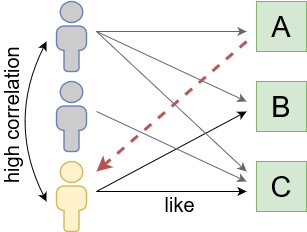
\includegraphics[scale=0.5]{images/UB_CF_ex.PNG}
	\caption{Esempio di applicazione di un sistema di raccomandazione User-based}
	\label{fig:UB_CF}
\end{figure}

Questi approcci sono facilmente implementabili, indipendenti dal contesto in cui sono applicati e possono essere più accurati rispetto
a tecniche basate sul content-based dall'altra parte all'aumentare del numero di utenti che vado a considerare per fare le 
raccomandazioni migliore è la precisione di questo processo ma anche è maggiore il costo per compiere questo procedimento. Altro 
problema che affligge questi sistemi, e che verrà approfondito nel prossimo paragrafo, è definito di Cold-start. 

\subparagraph{Item-based filtering} \hfill \break


Quando viene applicato per milioni di utenti e item, l'algoritmo UB-CF non è molto efficente, per via della complessa computazione della 
ricerca di utenti simili; così in alternativa è stato introdotto l'algoritmo di filtraggio Item-based, definito anche IB-CF 
(\textit{Item-based Collaborative Filter}): dove piuttosto che effetuare il confrotto tra utenti simili, viene fatto un confronto tra 
gli item dell'utente a cui si vule raccomandare e i possibili item simili.

Questi sistemi sono estremamente simili ai sistemi di raccomandazione Content-based, e identificano item simili in base a come utenti gli
hanno usati nel passato.


\cite{item-based-collaborative-filtering}

\begin{figure}[ht!]
	\centering
	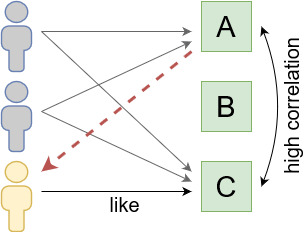
\includegraphics[scale=0.5]{images/IB_CF_ex.PNG}
	\caption{Esempio di applicazione di un sistema di raccomandazione Item-based}
	\label{fig:IB_CF}
\end{figure}

\paragraph{Model-based filtering}



Model-based algorithm tries to compress huge database into a model and 
performs recommendation task by applying reference mechanism into this model. Model-based CF can response 
user’s request instantly. This paper surveys common techniques for implementing model-based algorithms. We 
also give a new idea for model-based approach so as to gain high accuracy and solve the problem of sparse 
matrix by applying evidence-based inference techniques. 

\subsection{Challenges and limitations} \hfill \break



Cold start problem
What will happen if a new user or a new item is added in the dataset? It is called a Cold Start. There can be two types of cold start:
	Visitor Cold Start: means that a new user is introduced in the dataset. Since there is no history of that user, the system does not 
know the preferences of that user. It becomes harder to recommend products to that user. So, how can we solve this problem? One basic
approach could be to apply a popularity based strategy, i.e. recommend the most popular products. These can be determined by what has
been popular recently overall or regionally. Once we know the preferences of the user, recommending products will be easier.
	Product Cold Start: means that a new product is launched in the market or added to the system. User action is most important to
determine the value of any product. More the interaction a product receives, the easier it is for our model to recommend that product
to the right user. We can make use of Content based filtering to solve this problem. The system first uses the content of the new 
product for recommendations and then eventually the user actions on that product.


  Cons
	Scalability: The more K neighbors we consider (under a certain threshold), the better my classification should be. 
  Nevertheless, the more users there are in the system, the greater the cost of finding the nearest K neighbors will be.
	Cold-start: New users will have no to little information about them to be compared with other users.
	New item: Just like the last point, new items will lack of ratings to create a solid ranking (More of this on ‘How to sort 
  and rank items’).

Sparsity
Stated simply, most users do not rate most items and, hence, the user ratings matrix is typically very sparse. is is a problem for 
collaborative +ltering systems, since it decreases the probability of +nding a set of users with similar ratings. This problem often 
occurs when a system has a very high item-to-user ratio, or the system is in the initial stages of use. This issue can be mitigated by 
using additional domain information or making assumptions about the data generation process that allows for high-quality imputation.

